\chapter{测试部分}

\section{前端测试}
\subsection{集中测试}
采用testCafe工具对页面和组件进行测试,该组件可以通过npm指令安装,同时支持chrome浏览器和firefox浏览器,他可以在这两个浏览器上对代码进行测试。测试前需要保证安装有chrome或者firefox浏览器。
TestCafe安装方法:
\begin{itemize}
    \item npm install -g testcafe
    \item 安装时可以在elmclient目录下执行这个命令
    \item 然后就可以在elmclient目录下编写测试代码并通过执行
    \item testcafe 浏览器名 测试代码文件名
\end{itemize}
运行测试代码。例如:
testcafe chrome alert-test.js,
使用chrome浏览器运行alert-test.js文件,
首先测试backer,测试成功:
    \begin{figure}[H]
        \centering
        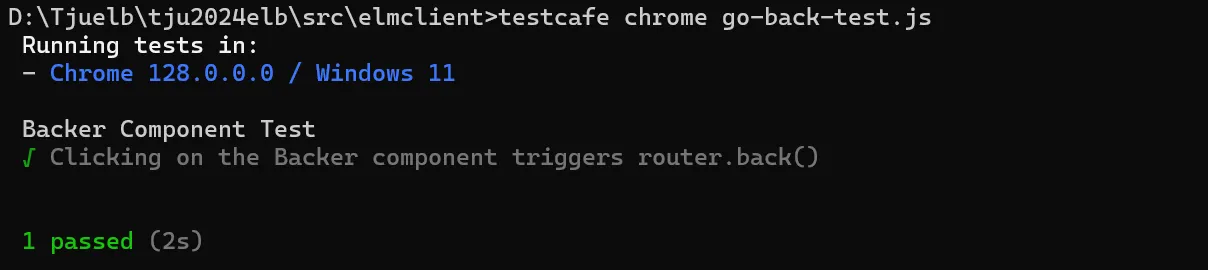
\includegraphics[width=0.75\linewidth]{pics/test1.png}
    \end{figure}













\section{后端测试}
添加h2内嵌数据库和mybatis-spring-boot-starter-test依赖,来进行后端单元测试

\begin{enumerate}


\item 设置测试环境:
\begin{itemize}
    \item @SpringBootTest 注解:告诉 Spring Boot 测试框架这是一个 Spring Boot 应用的测试类,它会启动应用上下文。
    \item @Autowired 注解:自动注入测试实例
    \item @MockBean 注解:创建测试实例调用的模拟对象。在测试中不调用实际的实现,而是使用模拟对象来控制行为和返回值。
\end{itemize}


\item 测试数据准备
\begin{itemize}
    \item 以BusinessService的ListBusinessByOrderTypeId为例,创建三个 `Business` 对象,分别设置它们的 `orderTypeId` 和 `businessName` 属性。
    \item 根据 `orderTypeId` 将 `Business` 对象分组到两个列表中,模拟数据库查询的结果。
\end{itemize}


\item  设置预期行为
\begin{itemize}
    \item 使用 Mockito 的 `when(...).thenReturn(...)` 方法设置模拟对象的预期行为。
    \item 当 `listBusinessByOrderTypeId` 方法被调用时,根据传入的 `orderTypeId` 返回相应的商家列表。
\end{itemize}


\item 执行操作

\begin{itemize}
    \item 调用 `businessService.listBusinessByOrderTypeId` 方法两次,分别传入不同的 `orderTypeId`,获取结果列表。
\end{itemize}

\item  验证结果

\begin{itemize}
    \item 使用 `assertNotNull` 验证返回的列表不为 `null`。
    \item 使用 `assertEquals` 验证返回的列表与预期的列表相等。
    \item 使用 `assertNotEquals` 验证两个不同 `orderTypeId` 返回的列表不相等。
\end{itemize}

\item  验证交互


\begin{itemize}
    \item 使用 Mockito 的 `verify` 方法验证 `businessServiceImpl` 是否被正确调用了 `listBusinessByOrderTypeId` 方法,并且传入了正确的参数。

    \item 这个测试类确保了 `BusinessService` 的 `listBusinessByOrderTypeId` 方法能够根据订单类型 ID 正确地返回商家列表,并且能够处理不同的输入。
    \item 对于controller层,由于添加了token验证,拦截器会拦截所有不在排除路径中的,token不符的url,使用@MockBean注解TokenInterceptor以绕过拦截器,便于controller层测试
\end{itemize}

\end{enumerate}



